\documentclass{article}
\usepackage{caption}
\usepackage{graphicx}
\usepackage[margin=1.5in]{geometry}
\usepackage{listings}
\usepackage{amsmath}

\newcommand\email{andredbsc@gmail.com}
\newcommand\discord{dbsc\#3718}

\title{ZK University \\[4pt] \normalsize\textsc{Week 2 Submission}}
\author{André Dal Bosco \\ \small{\email \quad \discord}}

\begin{document}
\maketitle

1.1 \begin{itemize}
    \item Gas cost: SHA256 $<$ Poseidon $<$ Pedersen $\simeq$ MiMC
    \item Capacity: SHA256 $\simeq$ MiMC $<$ Poseidon $\simeq$ Pedersen
    \item Proof generation efficiency: SHA256 $\simeq$ MiMC $<$ Pedersen $\simeq$ Poseidon
    \item Proof size: SHA256 $\simeq$ Poseidon $\simeq$ MiMC $\simeq$ Pedersen
\end{itemize}

References: \begin{itemize}
    \item https://github.com/iden3/circomlib/blob/master/circuits/poseidon.circom
    \item https://github.com/iden3/circomlib/blob/master/circuits/pedersen.circom
    \item https://github.com/iden3/circomlib/blob/master/circuits/mimc.circom
    \item https://github.com/iden3/circomlib/blob/master/circuits/sha256/sha256.circom
    \item https://medium.com/aztec-protocol/plonk-benchmarks-ii-5x-faster-than-groth16-on-pedersen-hashes-ea5285353db0
    \item https://medium.com/aztec-protocol/plonk-benchmarks-2-5x-faster-than-groth16-on-mimc-9e1009f96dfe
\end{itemize}

\begin{figure}[h]
    \centering
    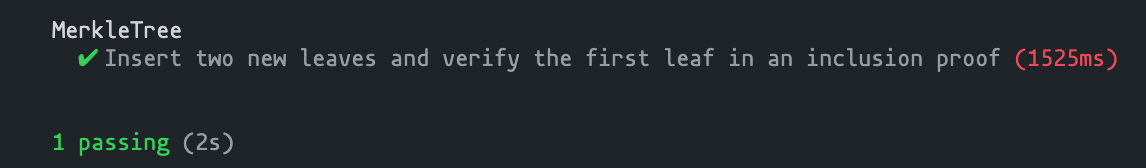
\includegraphics[width=0.75\textwidth]{img1.png}
    \caption*{Tests of task 1.2.}
\end{figure}


2.1 Tornado Cash Nova allows one to deposit a unspecified amount of ETH, while Tornado Classic only allows certain amounts to be deposited.

2.2 Relayers are needed because if one needs to pay fees do withdraw, in the process of obtaining the means to pay these fees they may link themselves with the final address that will receive the money. Because of this, it is better if someone else pays for these fees --- the relayers.

\begin{figure}
    \centering
    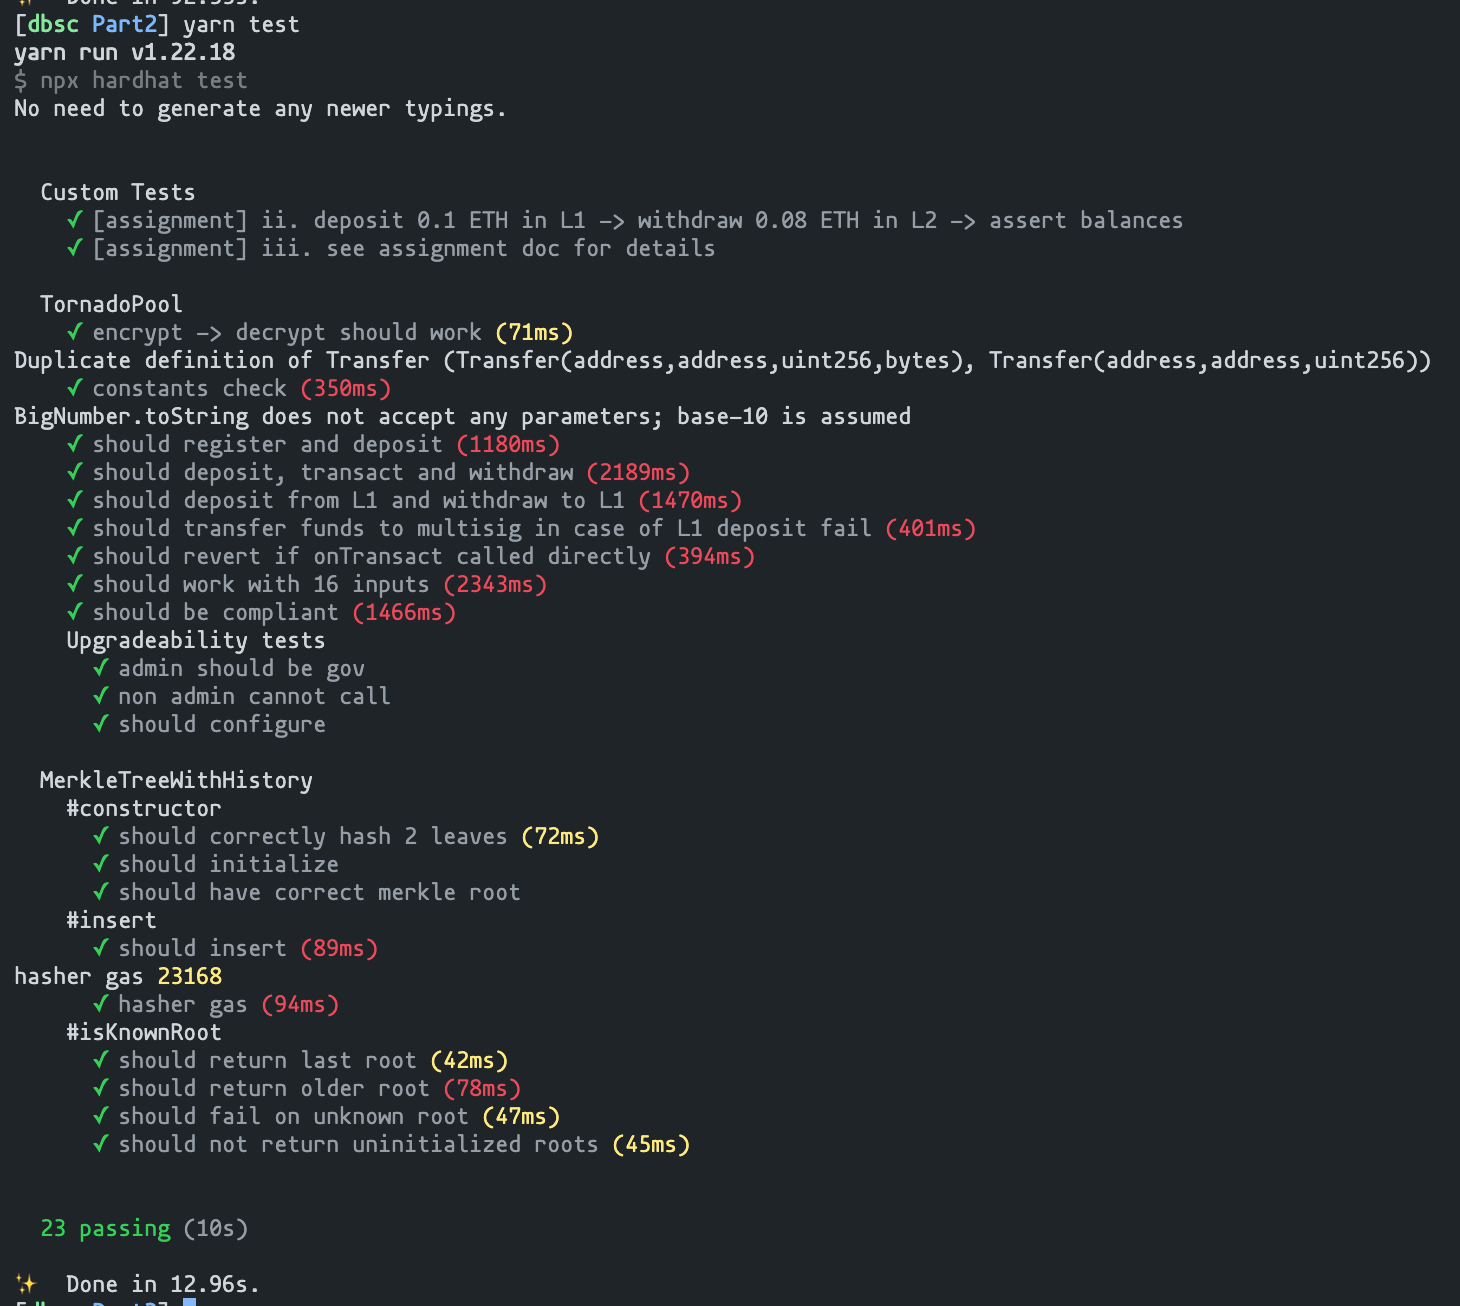
\includegraphics[width=0.75\textwidth]{img2.png}
    \caption*{Tests of task 2.3.}
\end{figure}

3.1 Semaphore is basically a system where users to prove they make part of set of registered identities, and signal their endorsement of an arbitrary string in a way that there can be no double signals.

3.2 Double signing is prevented via a external nullifier, which can be the address of a relevant smart contract, or hash of a URL, between other possibilities. If a signal is broadcasted more than one time to a given external nullifier, it is rejected.

3.3 It could be used to provide access to events in a way that the given ticket cannot be double spended, and from the ticket it is not possible to figure out who is the attendee. Maybe it could also be used to claim airdrops from NFTs in a way that no information about your NFT is surrendered, but at the same time, the airdrop will be clamable only once.
\end{document}
